\section{Analysis}
\label{sec:analysis}
\begin{algorithm}
\SetAlgoLined
\textbf{Input:} G(V, E), directed graph\\
\textbf{Output:} G$'$(V, E$'$), undirected graph\\
\textbf{Auxillary Functions:} \\
(a)$Pos(X)$: $+ve$ messages $\in$ X, \\
(b) $Neg(X)$: $-ve$ messages $\in$ X, \\
(c) $Polarity((x, y))$: assign polarity to edge $(x, y)$\\ 
\textbf{Initialize: }E$'$ = $\phi$\\
\For{$(u,v) \in E$}{
create $M$, the set of all messages in $(u, v)$\\
\If{$(v, u) \in E$}{ add all messages in $(v, u)$ to $M$}
\If{$|Pos(M)| = |Neg(M)| = 0$}{skip iteration}
\If{$|Pos(M)| \geq |Neg(M)|$}{$Polarity((u, v)) = +$}
\Else{$Polarity((u, v)) = -$}
$E' = E' \cup (u, v)$
}
\caption{Directed graph flattening}
\label{algo:directedToUndirected}
\end{algorithm}

Given the fact that we do not have complete messaging information from non-participants, we cannot consider all combinations of participant--non-participant triads. 
We define a triad to be \textit{valid} if it has at least two participants. 
All other forms of triads, with zero or one participant, are ignored from our consideration. 
\subsection{Balance Theory}
\begin{figure}[h]
\centering
\subfigure[$T_1$]{
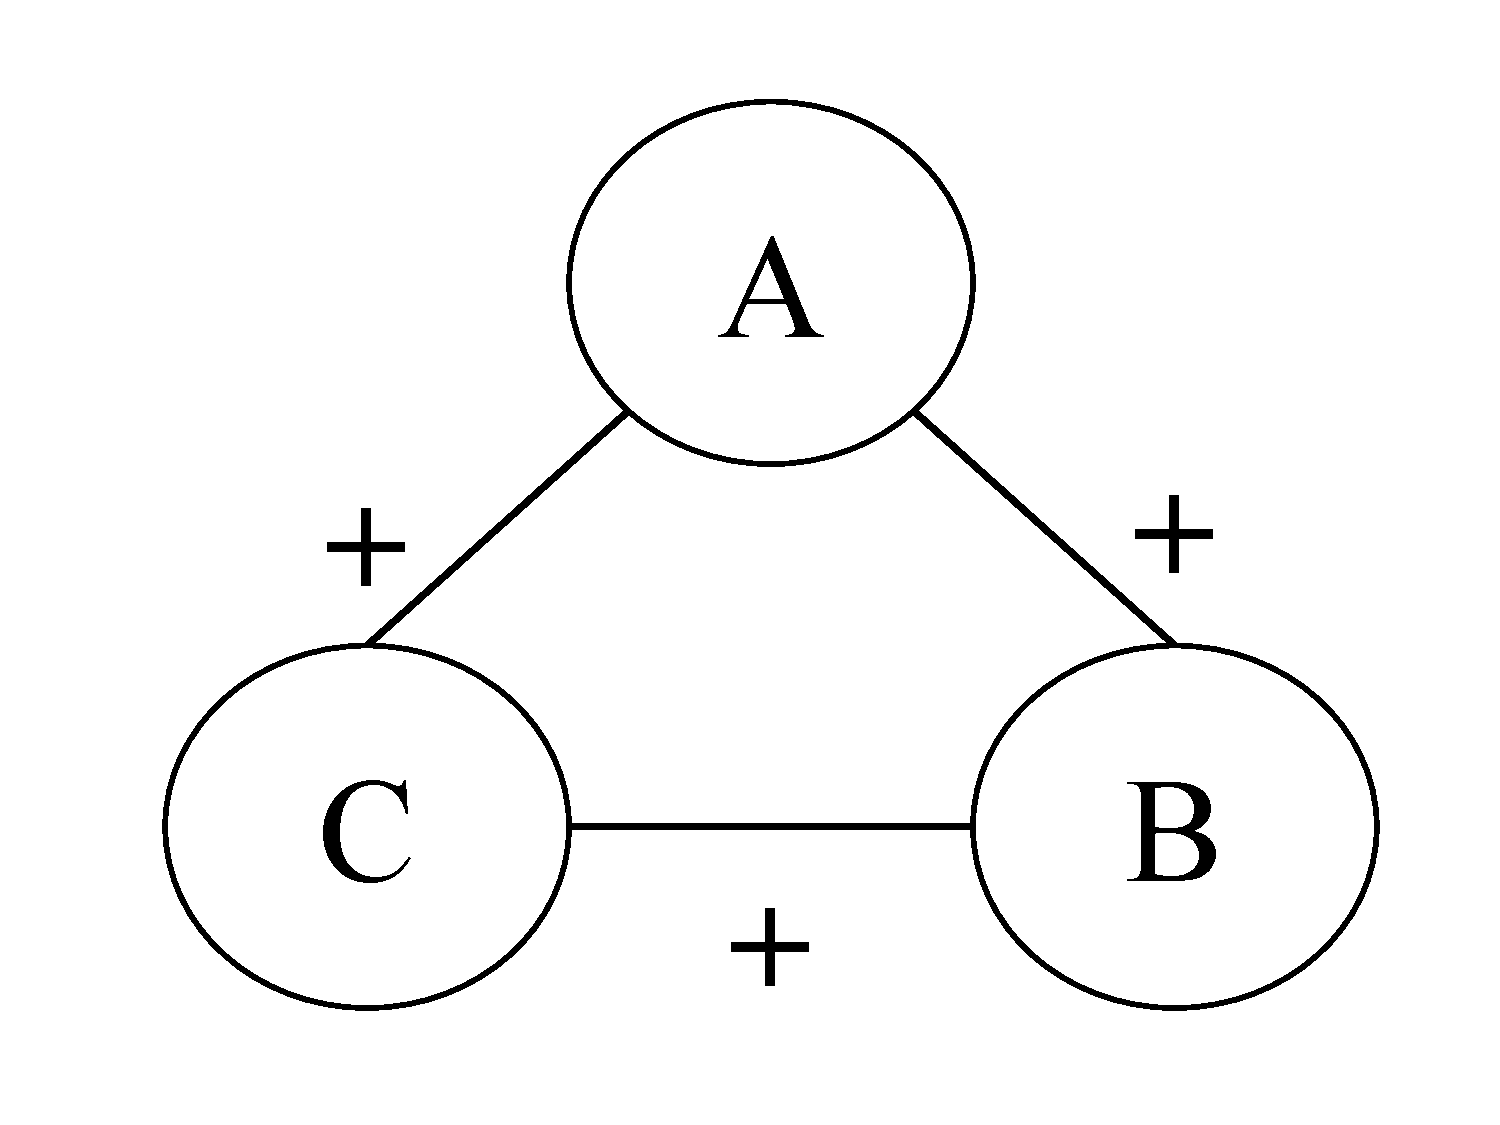
\includegraphics[scale=0.1]{balance_3P0N.pdf}
\label{fig:balance_3P0N}
}
\quad
\subfigure[$T_2$]{
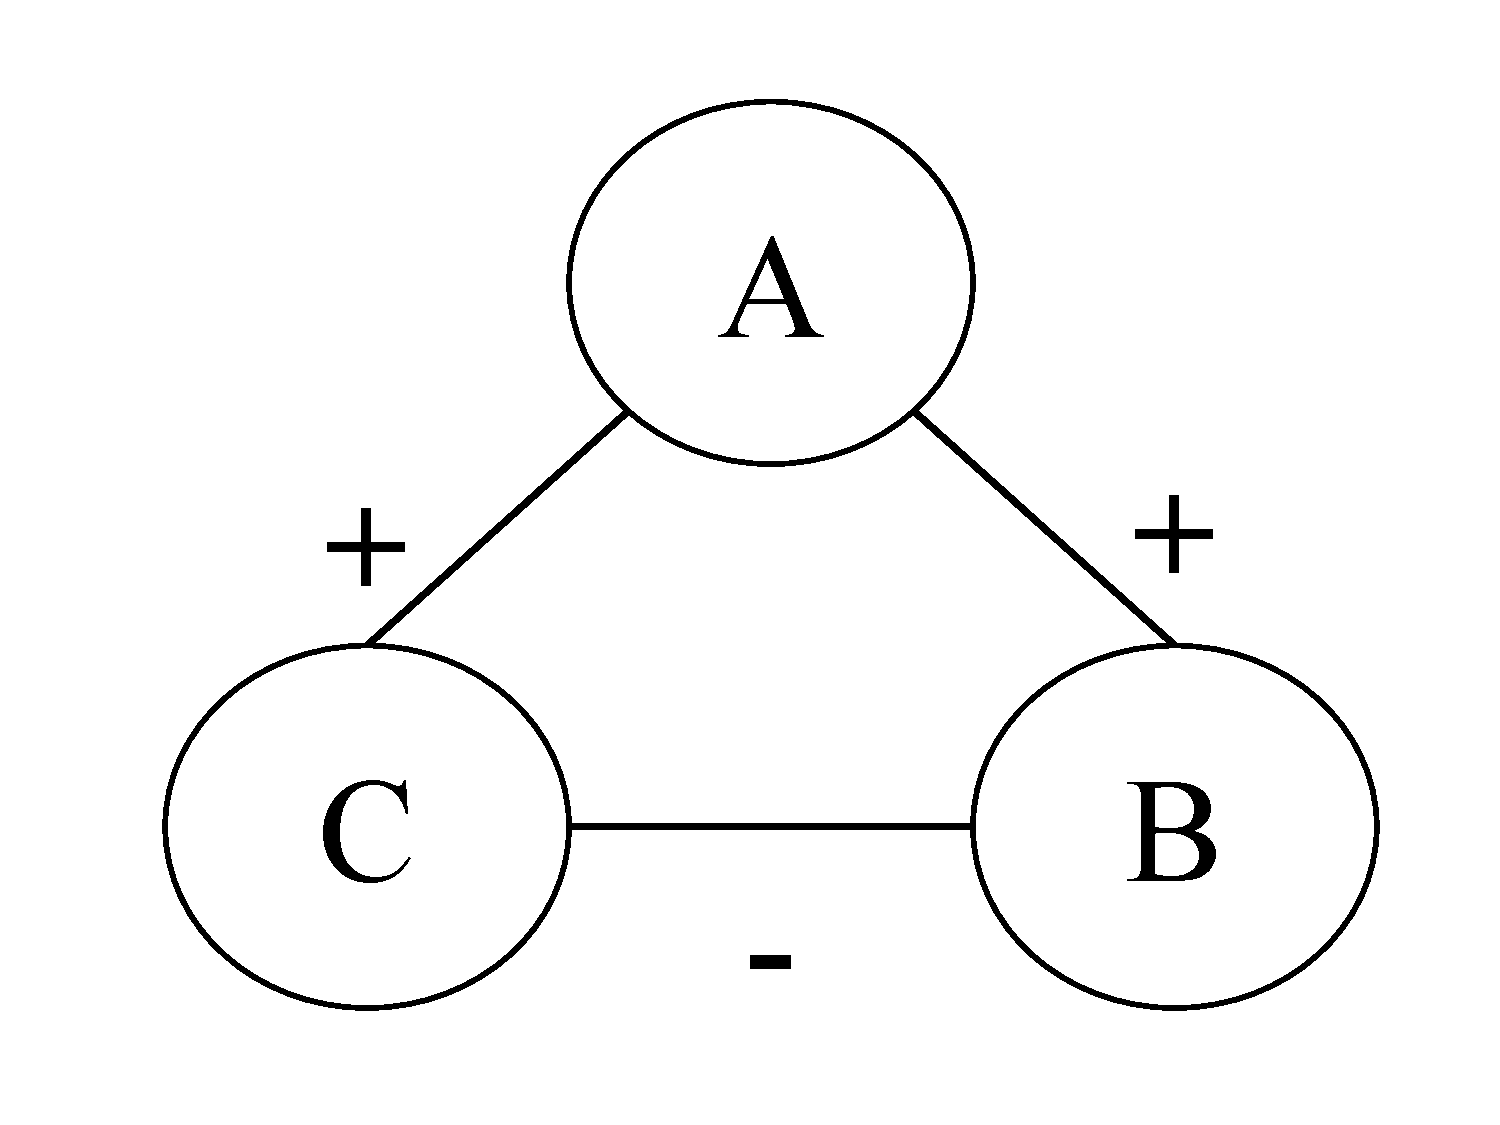
\includegraphics[scale=0.1]{balance_2P1N.pdf}
\label{fig:balance_2P1N}
}

\subfigure[$T_3$]{
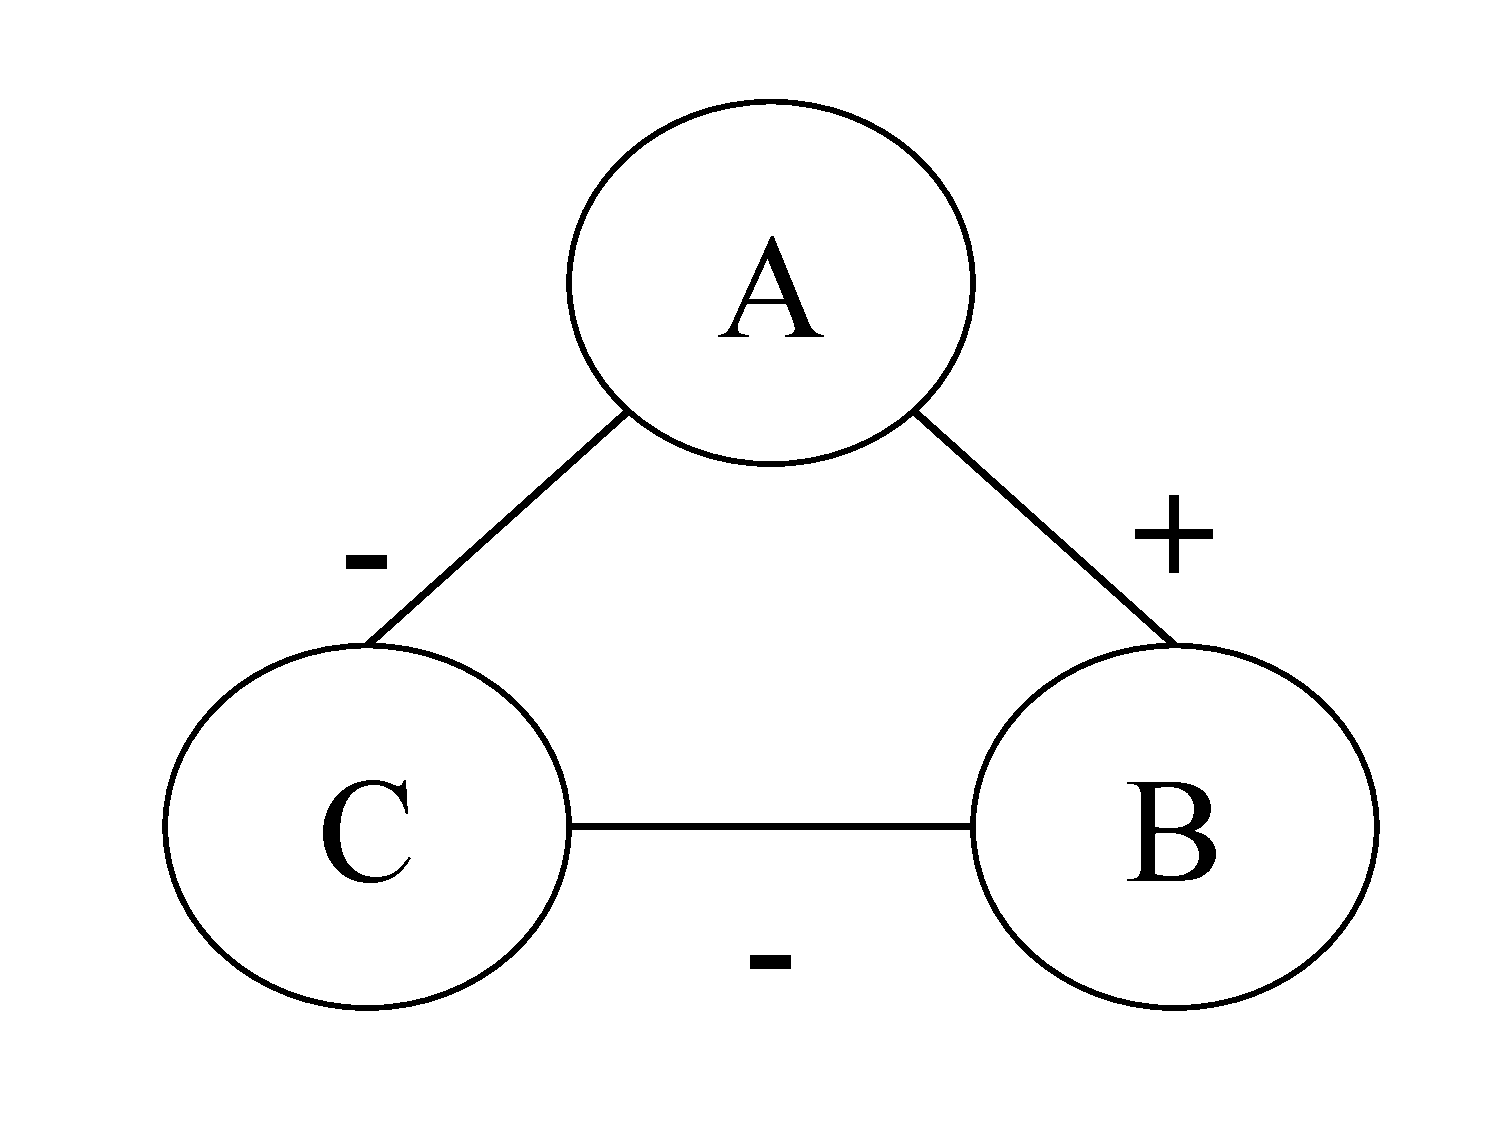
\includegraphics[scale=0.1]{balance_1P2N.pdf}
\label{fig:balance_1P2N}
}
\quad
\subfigure[$T_4$]{
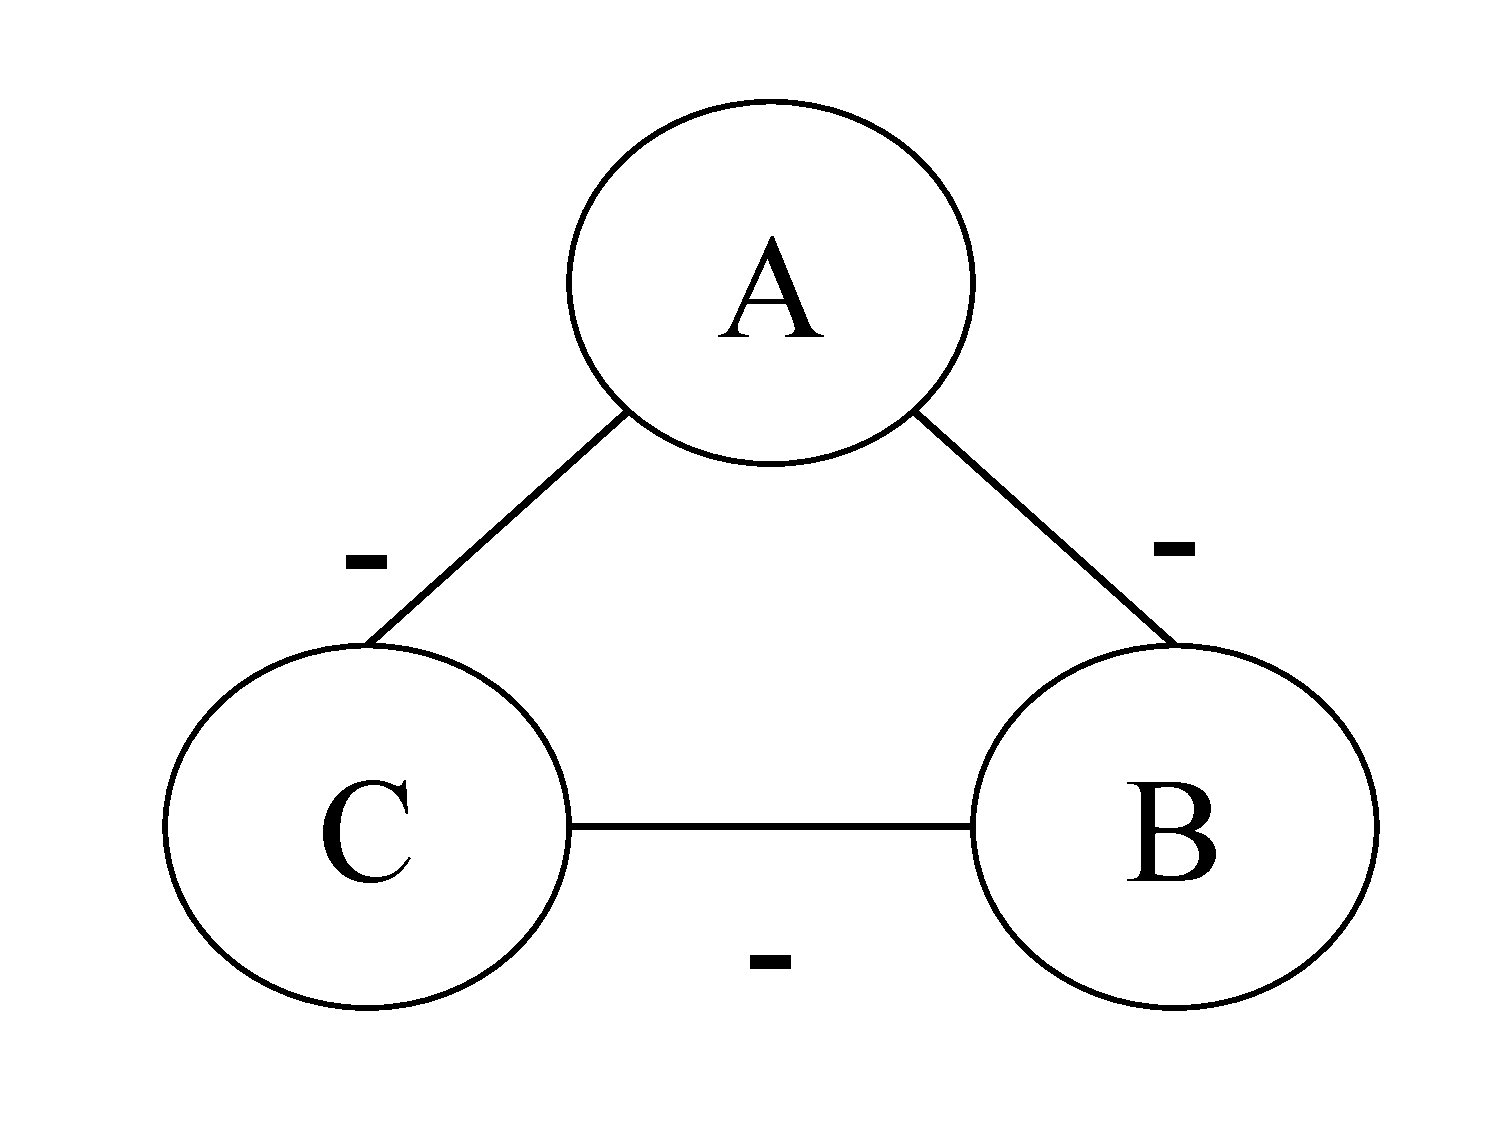
\includegraphics[scale=0.1]{balance_0P3N.pdf}
\label{fig:balance_0P3N}
}
\caption{Signed triads from balance theory. Triads $T_1$, and $T_3$ are \textit{balanced}, while triads $T_2$, and $T_4$ are \textit{unbalanced}}
\label{fig:balanceT}
\end{figure}

We investigated the structural compliance of our social network with \textit{structural balance theory} proposed by Heider in \cite{heider1946attitudes}. 
This theory was recast in a graph-centric manner by Cartwright and Hararay\cite{cartwright1956structural}. 
The theory describes the states in which signed triads can exist (see Figure \ref{fig:balanceT}). 
It also puts forward the idea that certain types of triads are more likely to occur than others in real social networks. 
Specifically, triads $T_1$ (Fig. \ref{fig:balance_3P0N}) and $T_3$ (Fig. \ref{fig:balance_1P2N}) are more likely, and are commonly referred to as \textit{balanced} triads. 
While triads $T_2$ and $T_4$ are less likely to occur, and are known as \textit{unbalanced} triads. 
Intuitively, $T_1$ and $T_3$ can be thought of espousing the ideas that \emph{a friend of a friend is my friend}, and \emph{enemy of my enemy is my friend respectively}. 
While, $T_2$ and $T_4$ can be understood by casting them as \emph{my enemy and I have a common friend}, and \emph{my enemy and I have a common enemy} respectively. 
An important underlying assumption for these triads is that the graph is undirected. 
Our dataset is inherently a directed graph with edge direction denoting the direction message flow between the nodes.
In order to make the analysis compatible with the theory we need to convert the network into an undirected graph. 
We use Algorithm \ref{algo:directedToUndirected} for this conversion which assigns the edge label using a majority based rule. 
The dataset is analyzed in two way: (i) \emph{overall}: we evaluate the compliance for the dataset across the length of the study, and (ii) \emph{monthly}: we also evaluate the evolution of the the structural properties on a monthly basis.

\subsubsection{\textbf{Overall Analysis}}
\begin{table}[!ht]
\centering
% balance theory overall - AFINN
%('P', 'P', 'N') Study:  0.358974358974 ( 28 )  Random:  0.423076923077 ( 33 )
%('P', 'P', 'P') Study:  0.269230769231 ( 21 )  Random:  0.24358974359 ( 19 )
%('N', 'N', 'N') Study:  0.0897435897436 ( 7 )  Random:  0.0769230769231 ( 6 )
%('P', 'N', 'N') Study:  0.282051282051 ( 22 )  Random:  0.25641025641 ( 20 )
\caption{Distribution of Balanced and Unbalanced Triads}
\begin{tabular}{| c | c | c |}
\hline
\textbf{Triad Type($T_i$)} & \textbf{$d_i$} & \textbf{$r_i$} \\
\hline
$T_1$ ($+++$) & 0.27 (21) & 0.244 (19)\\
\hline
$T_2$ ($++-$) & 0.359 (28) & 0.423 (33)\\
\hline
$T_3$ ($+--$) & 0.282 (22) & 0.256 (20)\\
\hline
$T_4$ ($---$)& 0.089 (7) & 0.077 (6)\\
\hline
\end{tabular}
\label{table:balanceTDist}
\end{table}
We start our analysis by taking a bird's eye view of the network, to get a general understanding of the structural properties associated with our network. 
We check the prevalence of the different types of triads ($T_{1-4}$) in our network, and evaluate their conformity with Heider's theory. 
For such an evaluation, we generate another social network where the structure is exactly the same as our network but the polarities have been generated randomly using the same underlying distribution as our network. 
This methodology enables us to check how well does our data, derived from a real social network, on comparison with a randomly generated network fit the theorised model. 
Once the undirected version of the network has been obtained (using Algorithm \ref{algo:directedToUndirected}), we find the distribution of all the valid triads in our network ($d_i$), and the randomly generated network ($r_i$). 
The distributions are summarized in Table \ref{table:balanceTDist}. 

The analysis of the balanced triads, $T_1$ and $T_3$, reveals that they are more frequent, or \textit{over-represented} (as in \cite{Leskovec:2010hw}, in our network. 
This is in harmony with Heider's theory which posits that $T_1$ and $T_3$ are more likely to occur in real social networks. $T_1$ occurs more frequently by about 11\%, while $T_3$ occurs more frequently by 10\%. 
The analysis of the unbalanced triads, $T_2$ and $T_4$, presents mixed results. 
$T_2$ occurs less frequently, or is \textit{under-represented} (as in \cite{Leskovec:2010hw}), in our network in-line with Heider's theory. 
However, $T_4$ is more frequent (by almost 15\%) in our network, contradicting one of the tenets of balance theory. 
Overall we see that triads $T_1, T_2, $and $T_4$ are more frequent while $T_3$ is less frequent when compared with the random network which only partly conforms to balance theory. 
If we turn our focus to \emph{weak} structural balance, as proposed by Davis in 1967 \cite{Davis1967Clustering}, where the only implausible triad is $T_3$, we observe that our network conforms to this theory in its entirety. 

\textbf{Result}: \textit{The network as a whole only partly conforms with balance theory, but conforms with the idea of weak structural balance in its entirety.}
\newline
\subsubsection{\textbf{Monthly Analysis}}
\begin{table*}
\centering
\caption{Bi-Monthly distribution of balanced and unbalanced triads}
\label{table:balanceMDist}
\begin{tabular}{c|c|c|c|c|c|c|}
\cline{2-7}
 & \multicolumn{2}{c|}{\textbf{Months 1-2}} & \multicolumn{2}{c|}{\textbf{Months 3-4}} & \multicolumn{2}{c|}{\textbf{Months 5-6}} \\ \hline
\multicolumn{1}{|c|}{\textbf{Triad Type}$\downarrow$} & $d_{i}^{12}$ & $r_{i}^{12}$ & $d_{i}^{34}$ & $r_{i}^{34}$ & $d_{i}^{56}$ & $d_{i}^{56}$ \\ \hline
\multicolumn{1}{|c|}{$T_1$ ($+++$)} & 0.667 (8) & 0.25 (3) & 0.172 (6) & 0.114 (4) & 0.444 (4) & 0.111(1) \\ \hline
\multicolumn{1}{|c|}{$T_2$ ($++-$)} & 0.083 (1) & 0.167 (2) & 0.114 (4) & 0.457 (16) & 0.444 (4) & 0.667 (6) \\ \hline
\multicolumn{1}{|c|}{$T_3$ ($+--$)} & 0.167 (2) & 0.333 (4) & 0.542 (19) & 0.429 (15) & 0.111 (1) & 0.111(1) \\ \hline
\multicolumn{1}{|c|}{$T_4$ ($---$)} & 0.083 (1) & 0.25 (3) & 0.172 (6) & 0.0 (0) & 0.0 (0) & 0.111 (1) \\ \hline
\end{tabular}
\end{table*}

Since the data is collected over a period of 6 months, it is natural to evaluate the network as an evolving entity where characteristics can be transient. 
We evaluate the network at a bi-monthly granularity, this ensures the availability of sufficient data.  
For each period, as in the case of the previous analysis, we calculate the distribution of valid triads, and also for a randomly generated network with the same distribution of edge polarity for the same period.  
The distributions have been summarized in Table \ref{table:balanceMDist}. 

\textit{Months 1-2}: The balanced triads have mixed conformity with balance theory; $T_1$ is more frequent by $\approx$ 17\%, while $T_3$ is less frequent than its random counterpart by 50\%. 
The unbalanced triads, $T_{2, 4}$, are less frequent by 50\% and 67\% respectively. 
The triads also do not hold when we test them for conformity with the idea of weak structural balance.

\textit{Months 3-4}: The balanced triads conform with the idea of being more likely in real social networks than random networks, $T_1$ and $T_3$ are more frequent by 50\% and $\approx$ 26\% respectively. 
The unbalanced triads, however, exhibit mixed conformity with $T_2$ being less frequent by 75\%, but $T_4$ being more frequent. 
Unlike Months 1-2, the network structure here models the idea of weak structural balance quite well with $T_{1,3,4}$ being more frequent, and $T_2$ being less frequent than their random counterpart. 

\textit{Months 5-6}: $T_1$ is more frequent, while $T_3$ is as frequent as its random counterpart. 
The unbalanced triads, $T_2$ and $T_4$, are less frequent than their random counterparts. 
Overall, the structure for this period does not conform with either balance theory, or weak structural balance theory. 

\textbf{Result}: \textit{The temporally divided network conforms with weak structural balance for one instance, and does not conform at all with Heider's theory of structural balance.}

\subsection{Status Theory}
The nature of our network, directed and evolving over time, is inherently different from the requirements of balance theories and its evaluation with these theories can be considered suboptimal for understanding the underlying properties associated with it. 
In this subsection, we explore our network as an evolving entity where relations can be transient in nature. 